\documentclass[10pt,twocolumn,letterpaper]{article}

\usepackage{cvpr}
\usepackage{times}
\usepackage{epsfig}
\usepackage{graphicx}
\usepackage{amsmath}
\usepackage{amssymb}

% Include other packages here, before hyperref.

% If you comment hyperref and then uncomment it, you should delete
% egpaper.aux before re-running latex.  (Or just hit 'q' on the first latex
% run, let it finish, and you should be clear).
\usepackage[breaklinks=true,bookmarks=false]{hyperref}

\cvprfinalcopy % *** Uncomment this line for the final submission

\def\cvprPaperID{****} % *** Enter the CVPR Paper ID here
\def\httilde{\mbox{\tt\raisebox{-.5ex}{\symbol{126}}}}

% Pages are numbered in submission mode, and unnumbered in camera-ready
%\ifcvprfinal\pagestyle{empty}\fi
\setcounter{page}{4321}
\begin{document}

%%%%%%%%% TITLE
\title{Convolution Neutral Network to detect Recyclable Materials}

\author{Hafsa Fatima\\
University of Texas at Arlington\\
Texas,USA\\
{\tt\small hafsa.fatima@mavs.uta.edu}
}

\maketitle
%\thispagestyle{empty}

%%%%%%%%% ABSTRACT
\begin{abstract}
The objective of this project is to predict the waste item in an image based on the material using Convolution Neural network (CNN). The output of classifier is paper, metal, plastic, cardboard, glass and non-recyclable material. So, the material is not just classified based on how effectively it can be recycled but it also reject the objects that have contamination and non-recyclable. The paper investigates and compares different CNN architectures used to get accurate predictions.  Finally, the goal is to build a model that can not only help in efficient segregation but also detect anomaly like contamination, oily containers etc. This model can be used by recycling centers or at home as an initiative towards sustainable livelihood.
\end{abstract}
%%%%%%%%% BODY TEXT
\section{Introduction}
It is estimated that, by the end of the 2050, more than 2 billion tonnes of waste will be produced by humans. Therefore, cost to implement waste management by year 2020 will be 400 billion Dollars . Improper waste management will have enormous adverse impacts on the economy, the public health, and the environment \cite{1}. The waste in landfills contribute to greenhouse gases thus causing a vicious cycle of pollution, global warming and climate change.

In the wake of recent knowledge about climate change, the need for sustainable lifestyle is more essential than ever before. It is often said that “It is better not recycle at all, than to contaminate and not recycle properly”. Unfortunately, these contaminated loads are sent to the landfill instead of recycling centers because of contamination. The knowledge about proper recycling and segregation is not common among people. Moreover, Many do not recycle items even though they are recyclable due to lack of awareness. So instead, relying on technology can be beneficial to  recycle properly.

The recent advancements in the field of deep learning has contributed to improvements in computer vision. Convolution neural network is the most widely used deep learning algorithm for its wide application on image classification. 
%-------------------------------------------------------------------------
\subsection{Data Set}

There are a total of 2060 training images and 490 testing images. The images have 3 RGB channels and they are resized to 224 X 224 pixels. There are 6 classes in the data set which are paper, plastic, metal, cardboard,glass and non-recyclable. The objective of the design is to create a model that detects different types of recycling material. Non-recyclable class has images that are commonly considered as recyclable but they are not. According to ' The New York Times' article on "6 Things you are recycling wrong"[2] highlights the misguided approach to recycling certain items that are used in day to day life. The author surveyed that 90 percent of pizza boxes trashed in recycling bags. Greasy pizza boxes are not recyclable. These items are included in non-recycle class. 
\begin{table}
\begin{center}
\begin{tabular}{|1|c|c|}
\hline
Labels & Train images & Test images\\
\hline\hline
Plastic & 374 & 108 \\
Non-Recycle & 124 & 36 \\
Paper & 484 & 110\\
Glass & 436 & 65\\
Cardboard & 339 & 64\\
Metal & 302 & 108\\
\hline
\end{tabular}
\end{center}
\caption{Data set with 6 labels.}
\end{table}

\subsection{Data Augmentation}

The images are randomly transformed by applying Image Data generator feature. The transformation includes horizontal flips, re-scaling, zoom-range, shear-range etc.


%------------------------------------------------------------------------
\section{Methods}

The project studies different architectures of the Convolution Neutral network.This determines experimentally the best CNN for the given data set. CNN is one of the widely used tool for image classification. Since the image data is single object neutral network, deep learning using CNN is used. CNN extracts features from images using convolution layers. Learning the features helps in predictions of labels of image.

%-------------------------------------------------------------------------
\subsection{Convolution Neural Network with AlexNet}

Alex Krizhevsky changed the world when he first won Imagenet challenged in 2012 using a convolutional neural network for image classification task. Alexnet achieved top-5 accuracy of 84.6\% in the classification task while the team that stood second had top-5 accuracy of 73.8\% which was a record breaking and unprecedented difference. Before this, CNNs (and the people who were working on it) were not so popular among computer vision community. However, the tables were turned after this. Soon, most of the computer vision researchers started working on CNN and the accuracy has improved significantly over last 4-5 years.

\subsubsection{Model}
This network consist of 7 layers including convolution and dense layers \cite{alexnet}. It has 60 Million Parameters which are trainable.In the publication,AlexNet had 5 convolution layers network with variable filters size and kernal size. The output was for 1000 classes. It is still a CNN with layers of Pooling, activation and Dropouts. Most of the paremeters comes from last fully connect layer. Two Dense layers with 4096 nodes and then these are connected to output layer with 1000 parameters. The Layers also include batch normalization
Therefore, it is a sequential model of Total params: 28,085,758 where Trainable params are 28,064,622 and Non-trainable params are 21,136.
\subsubsection{Observation}
While Training, the accuracy reached upto 94.19\% with a loss of 18.40\%. The Average accuracy while testing is approximately 58\% .The Predictions of the 6 classes are shown in confusion Matrix.
\begin{figure}[h!]
    \centering
    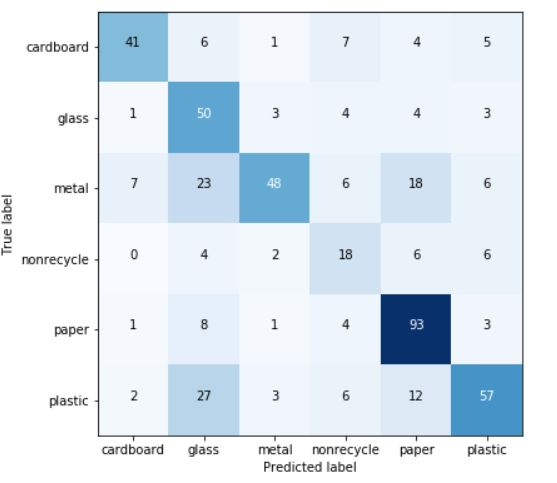
\includegraphics[scale=0.4]{pic/AlexCM.JPG}
    \caption{Confusion Matrix in AlexNet}
    \label{fig:Confusion Matrix in AlexNet}
\end{figure}

\subsection{Convolution Neural Network with VGGNet}
VGG which stands for Visual Geometry Group, was proposed by a reasearch group at Oxford in 2014\cite{VGGnet}. This network was once very popular due to its simplicity and some nice properties like it worked well on both image classification as well as detection tasks. In 2014, 16 and 19 layer networks were considered very deep (although we now have the ResNet architecture which can be successfully trained at depths of 50-200 for ImageNet and over 1,000 for CIFAR-10)\cite{internet}
\subsubsection{Model}
VGG has 19 layers and uses 3*3 convolution, in place of 11*11 convolution in Alexnet which works better as 11*11 in the first layer leaves out a lot of original information. Intially, the model is learnt at rate 0.002 to get to better accuracy faster. 
It is a sequential model with Total params: 134,285,126 out of which Trainable params are 24,582 and Non-trainable params are 134,260,544. This model is saved and then the learning rate is reduced to 0.0002. Now the model slowly moves towards optimal solution.

\subsubsection{Observation}
The training process reaches the accuracy of approximately 82\% and the testing average accuracy is 72\% (approx). The loss is around 0.47 w

\begin{figure}[h!]
    \centering
    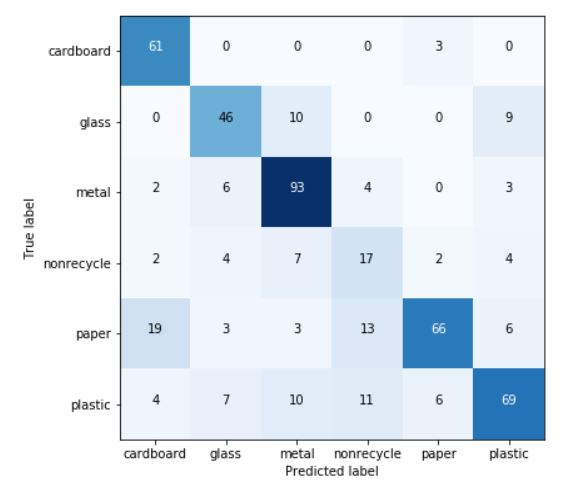
\includegraphics[scale=0.4]{pic/VGGCM.JPG}
    \caption{Confusion Matrix in VGGNet}
    \label{fig:Confusion Matrix in VGGNet}
\end{figure}

\subsection{Convolution Neural Network with MobileNet}
MobileNet is known for Depthwise Seperable Convolution and Light Weight Model. MobileNets are based on a streamlined architecture that uses depth-wise separable convolutions to build light weight deep neural network. networks.\cite{MobileNet}
\subsubsection{Model}
It is a sequential model with Total params: 4,253,864 out of which Trainable params: 4,231,976 and Non-trainable params: 21,888

\subsubsection{Observation}
The training process reaches the accuracy of approximately 81\% and the testing average accuracy is 72\% (approx).

\begin{figure}[h!]
    \centering
    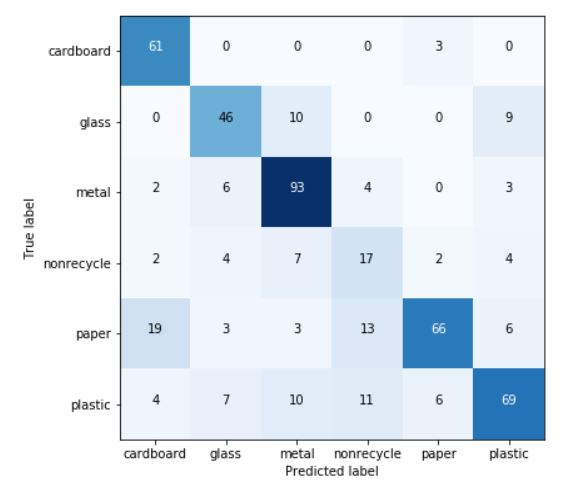
\includegraphics[scale=0.4]{pic/VGGCM.JPG}
    \caption{Confusion Matrix in VGGNet}
    \label{fig:Confusion Matrix in VGGNet}
\end{figure}

\subsection{Convolution Neural Network with ResNet}
ResNet is different from any traditional sequential CCN architectures such as AlexNet and VGG.\cite{ResNet} ResNet is a form of “state of the art architecture” that relies on micro-architecture modules (also called “network-in-network architectures”).\cite{internet}. ResNet architecture demonstrates that extremely deep networks can be trained using standard SGD (and a reasonable initialization function) through the use of residual modules:

\subsubsection{Model}
It is a huge network to network connection of layers with Total params: 25,874,932 out of which Trainable params: 261,132 and Non-trainable params: 25,613,800

\subsubsection{Observation}
The training process reaches the accuracy of approximately 74.61\% and the testing average accuracy is 58.12\% (approx).

\begin{figure}[h!]
    \centering
    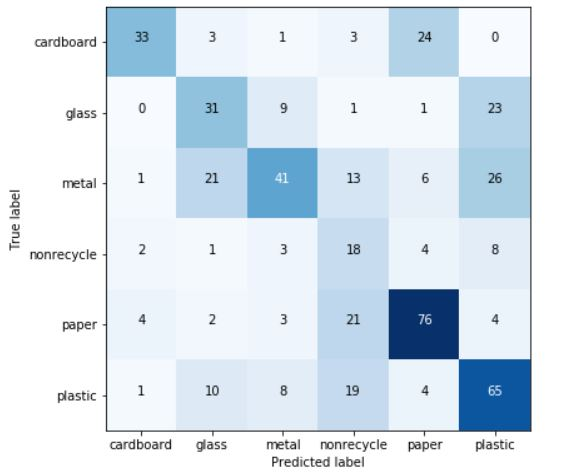
\includegraphics[scale=0.4]{pic/ResNetCM.JPG}
    \caption{Confusion Matrix in ResNet}
    \label{fig:Confusion Matrix in ResNet}
\end{figure}

%------------------------------------------------------------------------
\section{Result}
The most efficient model can be based on accuracy in training the CNN and accuracy in testing the model. The loss also plays a major factor in deciding when the model reaches its global minima. The model is gives the best predictions when it is at global minima.
\subsection{Accuracy VS Loss}
Comparing the Accuracy of different CNN gives a better idea of which model give most accurate prediction. From the Tables, VGGNet is well tuned in both training and testing.
\begin{table}[h!]
\begin{center}
\begin{tabular}{|1|c|c|}
\hline
Architectures & Accuracy & Loss\\
\hline\hline
AlexNet & 0.9419 & 0.1840 \\
VGGNet & 0.8205 & 0.4944 \\
ResNet & 0.718 & 0.81\\
MobileNet & 0.9216 & 0.2677\\
\hline
\end{tabular}
\end{center}
\caption{Accuracy and Loss in Training Models.}
\end{table}

\begin{table}[h!]
\begin{center}
\begin{tabular}{|1|c|c|}
\hline
Architectures & Accuracy & Loss\\
\hline\hline
AlexNet & 0.576 & 1.94734 \\
VGGNet & 0.7042 & 1.074 \\
ResNet & 0.57 & 1.74\\
MobileNet & 0.6500 & 2.18\\
\hline
\end{tabular}
\end{center}
\caption{Accuracy and Loss in Testing Models.}
\end{table}

\subsection{Size in terms of Parameter}
The parameters corresponds to neural nodes in the network. The amount of parameters matter when the prediction is done on a devices like phones. The more number of parameters, the longer it takes to compute predictions. The table shows MobileNet requires the least parameters. MobileNet id preferred in mobile devices.
\begin{table}[h!]
\begin{center}
\begin{tabular}{|1|c|c|c|}
\hline
Architectures & Total Params & Trainable  & Non-Traninable\\
\hline\hline
AlexNet & 28,085,758 & 28,064,622 & 21,136 \\
VGGNet & 134,285,126 & 24,582 & 134,260,544\\
ResNet & 25,874,932 & 261,132 & 25,613,800\\
MobileNet & 4,259,870 & 6,006 & 4,253,864\\
\hline
\end{tabular}
\end{center}
\caption{Parameters}
\end{table}
%------------------------------------------------------------------------
\section{Conclusion}
Waste Management is a huge problem for the environment. Using a deep leaning model can solve the basic need to recycle material. Recycling papers can save tons of trees that are used by the paper industry. Similarly, reusing metals can stop the extraction of minerals from earth. There are numerous benefits of recycling, but it can be a challenging task. Using deep learning models can reduce the complexity of Waste Management.
The experiment concludes that a model can be trained that effectively classifies objects in images into recyclable material or non-recyclable material. The observed models are going to be as good as the data given to it. The CNN model in VGGNet architecture gives the most efficient image classifier in terms of accuracy. MobileNet is the most efficient in terms of memory.
These models can be used by individuals to recycle items properly. It can also be used by recycling centers to predict the waste and segregate them with machinery automation and reduce the labor on humans.

\section{Future}
The next step would be to create a user interface to make the model more accessible. There is a need for more data to make better predictions. 
There are lot of benefits in using deep learning to solve these complex problems. Machines are faster and can help reduce manual annotation and segregation of recyclable material.It may not be the most accurate form of detection but it is close enough.

\begin{thebibliography}{9}
\bibitem{1} 
Kaza, Silpa; Yao, Lisa C.; Bhada-Tata, Perinaz; Van Woerden, Frank.
\textit{What a Waste 2.0: A Global Snapshot of Solid Waste Management to 2050}. 
World Bank, Washington, DC, USA,  2018.

\bibitem{alexnet} 
Alex Krizhevsky, Ilya Sutskever, Geoffrey E Hinton.
\textit{Imagenet classification with deep convolutional neural networks}. 
.\textit{Advances in neural information processing systems}.

\bibitem{VGGnet} 
Karen Simonyan & Andrew Zisserman.
[\textit{Karen Simonyan & Andrew Zisserman}]. Visual Geometry Group, Department of Engineering Science, University of Oxford, ICLR 2015.
 
 \bibitem{ResNet} 
Kaiming He, Xiangyu Zhang, Shaoqing Ren, Jian Sun.
\textit{Deep Residual Learning for Image Recognition}. 
The IEEE Conference on Computer Vision and Pattern Recognition (CVPR), 2016, pp. 770-778.

\bibitem{MobileNet} 
Andrew G. Howard, Menglong Zhu, Bo Chen, Dmitry Kalenichenko, Weijun Wang, Tobias Weyand, Marco Andreetto, Hartwig Adam.
\textit{MobileNets: Efficient Convolutional Neural Networks for Mobile Vision Applications}. 
The IEEE Conference on Computer Vision and Pattern Recognition (CVPR), 2017.

\bibitem{internet} 
Adrian Rosebrock: ImageNet: VGGNet, ResNet, Inception, and Xception with Keras,
\textit{https://www.pyimagesearch.com/2017/03/20/imagenet-vggnet-resnet-inception-xception-keras/}. 
\end{thebibliography}

\end{document}
